\documentclass{beamer}
\usepackage{ctex}
\usepackage{graphicx}

\usefonttheme[onlymath]{serif}% 数学公式字体设置

\usetheme{metropolis}
\title{整式}
\subtitle{Integral Expression}
\institute{Norsesun Milieu}
\author{K}
\date{\today}

\begin{document}
	\frame{\titlepage}
	
	\section{问题导入:代数式有什么特征?}
	\begin{frame}{代数式的特征}
		我们知道, $ 2x^2 + 3x - 1$, $ \dfrac{2x+1}{x} $ 这两个式子
		都是代数式,那么它们有什么不同的特征呢?
		
		\pause
		顾名思义, 从代数式的定义可知,代数式有两个主要特征
		
		1. 由字母或数组成
		
		2. 对于多个数或字母的代数式,它们之间由运算符号连接
	\end{frame}
	
	\section{代数式两种:单项式与多项式}
	\begin{frame}{单项式(Monomial)}
		\textbf{列代数式}
		
			1. 长为 $x$, 宽为 $0.8x$的长方形的面积是多少?
			
			2. 半径为 $r$ 的圆的面积是多少?
			
			3. 长方体的底面是边长为 $x$ 的正方形,高为 $y$, 它的体积是多少?
			\pause
			答:\\
				1. $0.8x^2$, 	\\
				2. $\pi r^2$, \\
				3. $x^2y$

	\end{frame}
	
	\begin{frame}{单项式的相关概念:Coefficient, Degree}
		像$0.8x^2$, $\pi r^2$, $x^2y$ 这样,由数与字母的\emph{积}组成的代数式叫做\\
		\textbf{单项式(Monomial)}。单独一个字母或一个数也是单项式。
		
		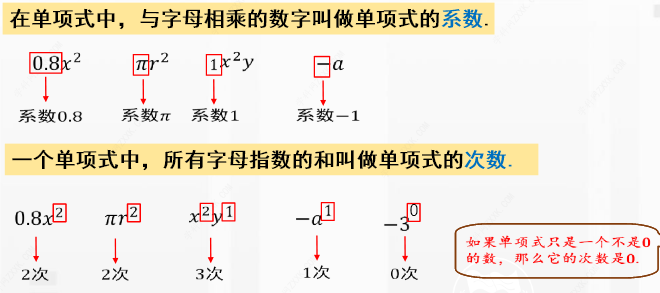
\includegraphics[width = .8\textwidth]{assets/monomial concepts.png}
	\end{frame}
	
	\begin{frame}{注意}
		\underline{单项式中字母不能作除数(分母)}, 如 $ \frac{1}{a}$ 就不是单项式,它是一个 				\textbf{分式}。 如同有理数分为整数与分数一样,整式和分式统称有理式。
		
		\vspace{2ex}
		圆周率 $\pi$ 是个常数,代表一个固定的量,当单项式中含有 $\pi$ 时,$\pi$ 是单项式系数			的组成部分。
		
		\vspace{2ex}
		单项式中字母的指数是 “$1$”时,“$1$” 省略不写,但在计算单项式的次数时,不能忽				略。比如 $-2x$ 这个单项式中 $x$ 的指数是 $1$,单项式的次数是 $1$。
	\end{frame}
	
	\begin{frame}{单项式概念的练习}
		1. 下列说法正确的是(  )\\
		\hspace{2ex}A. m 的系数是0 \\
		\hspace{2ex}B. $ \dfrac{1}{m}$是单项式 \\
		\hspace{2ex}C. $ -5x $ 的系数是5 \\
		\hspace{2ex}D. 0是单项式
		
		\vspace{3ex}
		2. 单项式 $-\dfrac{3}{2}x^2y^3$ 的系数是多少,次数是多少?
	\end{frame}
	
	\begin{frame}{判断}
		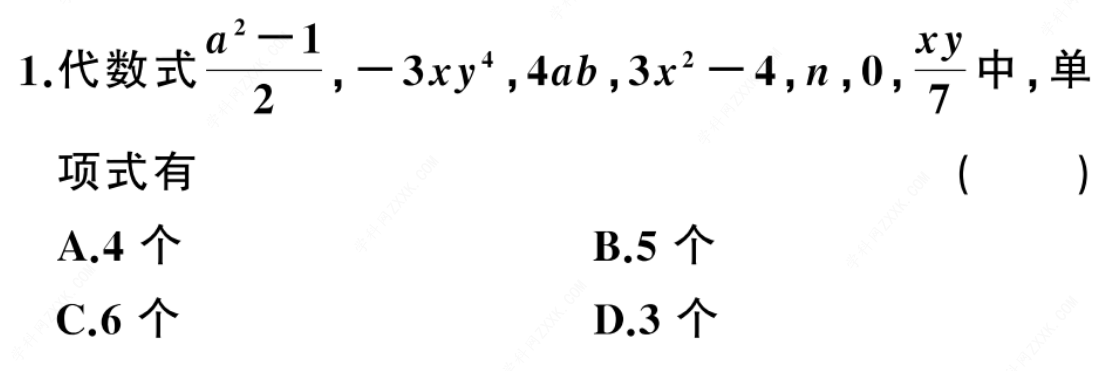
\includegraphics[width = .8\textwidth]{assets/monomial 2.png}
	\end{frame}
	
	\begin{frame}{多项式的相关概念:Term, Constant Term}
		几个单项式的和组成的代数式叫做 \textbf{多项式(Polynomial)}。
		
		\vspace{3ex}
		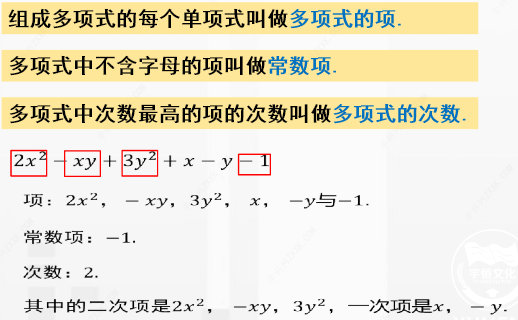
\includegraphics[width = .8\textwidth]{assets/polynomial.png}
	\end{frame}
	
	\begin{frame}{注意点}
		\textbf{多项式(Polynomial)}的项数与次数。
		
		\vspace{3ex}
		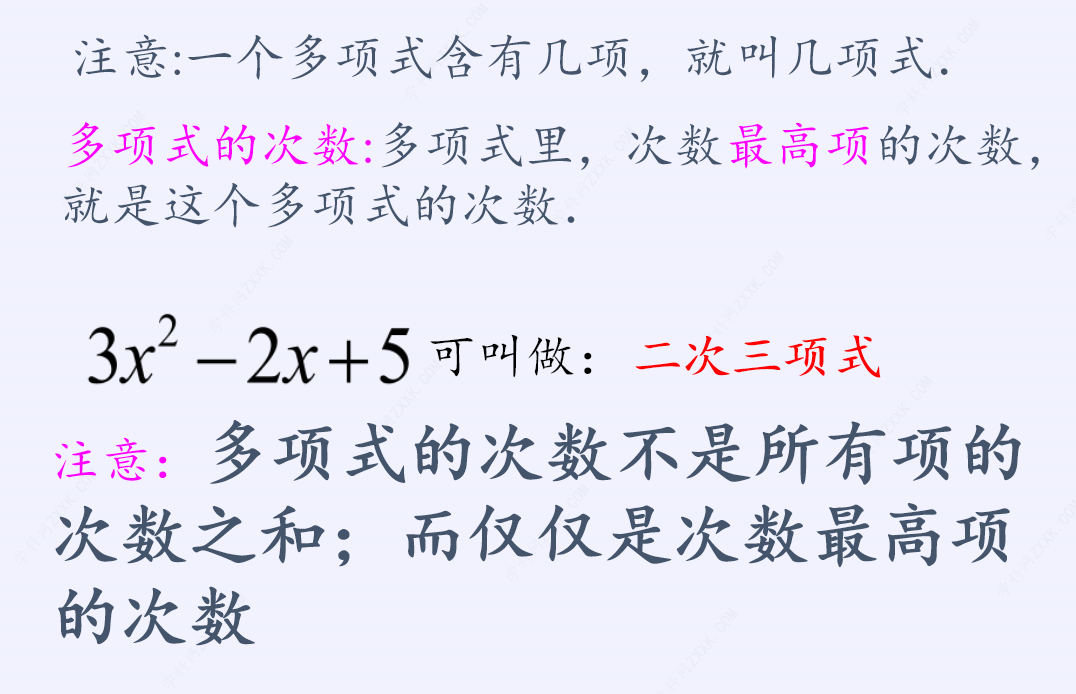
\includegraphics[width = .8\textwidth]{assets/polynomial attention.png}
	\end{frame}
	
	\begin{frame}{多项式练习}
		
		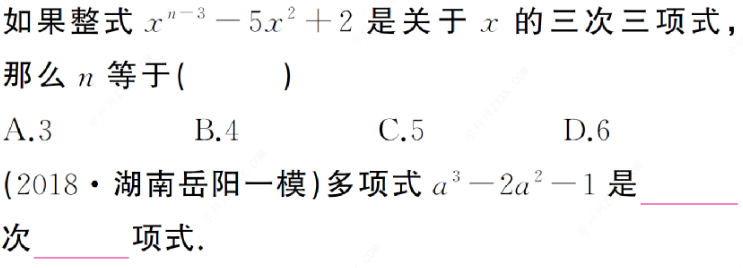
\includegraphics[width = .8\textwidth]{assets/polynomial practice.png}
	\end{frame}
	
	\begin{frame}{漂亮地排列多项式}
		
		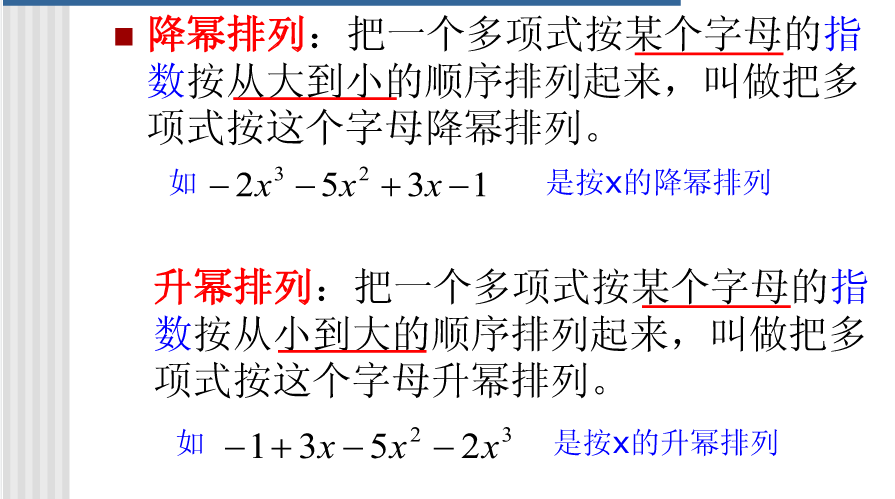
\includegraphics[width = .99\textwidth]{assets/polynomial 2.png}
	\end{frame}
	
	\begin{frame}{整式的概念}
		单项式和多项式统称为 \textbf{整式(Integral Expression)}。
	\end{frame}
	
	\begin{frame}{总结}
		什么是 \textbf{整式(Integral Expression)}?单项式的次数与系数怎么理解?多项式的次数怎么理解?
	\end{frame}
\end{document}